\pagestyle{azougue}
\label{azougue}


\begin{textblock*}{5.625in}(0pt,0pt)%
\vspace*{-1.45cm}
\hspace*{-1.8cm}\includegraphics*[width=112mm]{./imgs/AZOUGUE.png}
\end{textblock*}

\pagebreak

\hspace{.5cm}

\begin{center}
\hspace*{-2.5cm}\raisebox{5.5cm}{\rotatebox[origin=t]{90}{\Formular{\textbf{Lançamento}}}}
\hspace*{2cm}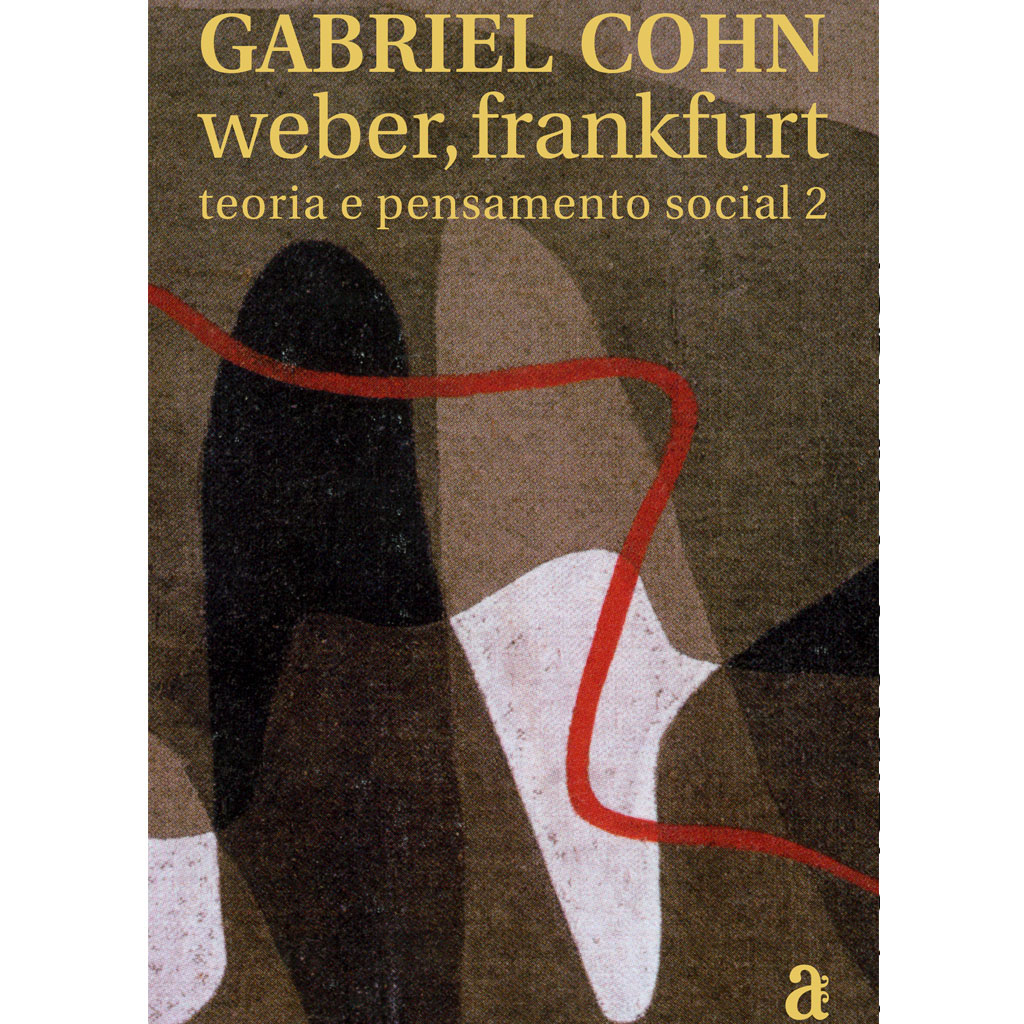
\includegraphics[width=45mm]{./imgs/weber.jpg}
\end{center}

\hspace*{-2cm}\_\_\_\_\_\_\_\_\_\_\_\_\_\_\_\_\_\_\_\_\_\_\_\_\_\_\_\_\_\_\_\_\_\_\_\_\_\_\_\_\_\_\_\_\_\_\_\_\_\_\_\_\_\_\_\_\_\_\_\_\_\_\_\_\_\_\_\_\_\_\_\_\_\_

\medskip

\noindent{}Essa coletânea de textos sobre questões sociológicas, políticas e culturais, escritos nas últimas décadas pelo sociólogo, cientista político e professor emérito da \scalebox{.8}{USP} Gabriel Cohn, traz estudos teóricos sobre pensadores internacionais de primeira linha, indo de Karl Marx a Florestan Fernandes passando por clássicos como Max Weber e Emile Durkheim e os autores da Escola de Frankfurt, junto com análises de problemas globais e da realidade brasileira, sobre questões fundamentais como as do desenvolvimento e da civilização.

%\hspace{.5cm}
\vfill

\hspace*{-.4cm}\begin{minipage}[c]{0.90\linewidth}
\small{
{\Formular{\textbf{
\hspace*{-.1cm}Título: Weber (Frankfurt 2)\\
Autor: Gabriel Cohn\\ 
Editora: Azougue\\
Páginas: 268\\
Formato: 17x24cm\\
Preço: R\$ 89,90\\
ISBN: 978-85-7920-235-3
}}}}
\end{minipage}

\pagebreak

\hspace{.5cm}

\begin{center}
\hspace*{-.5cm}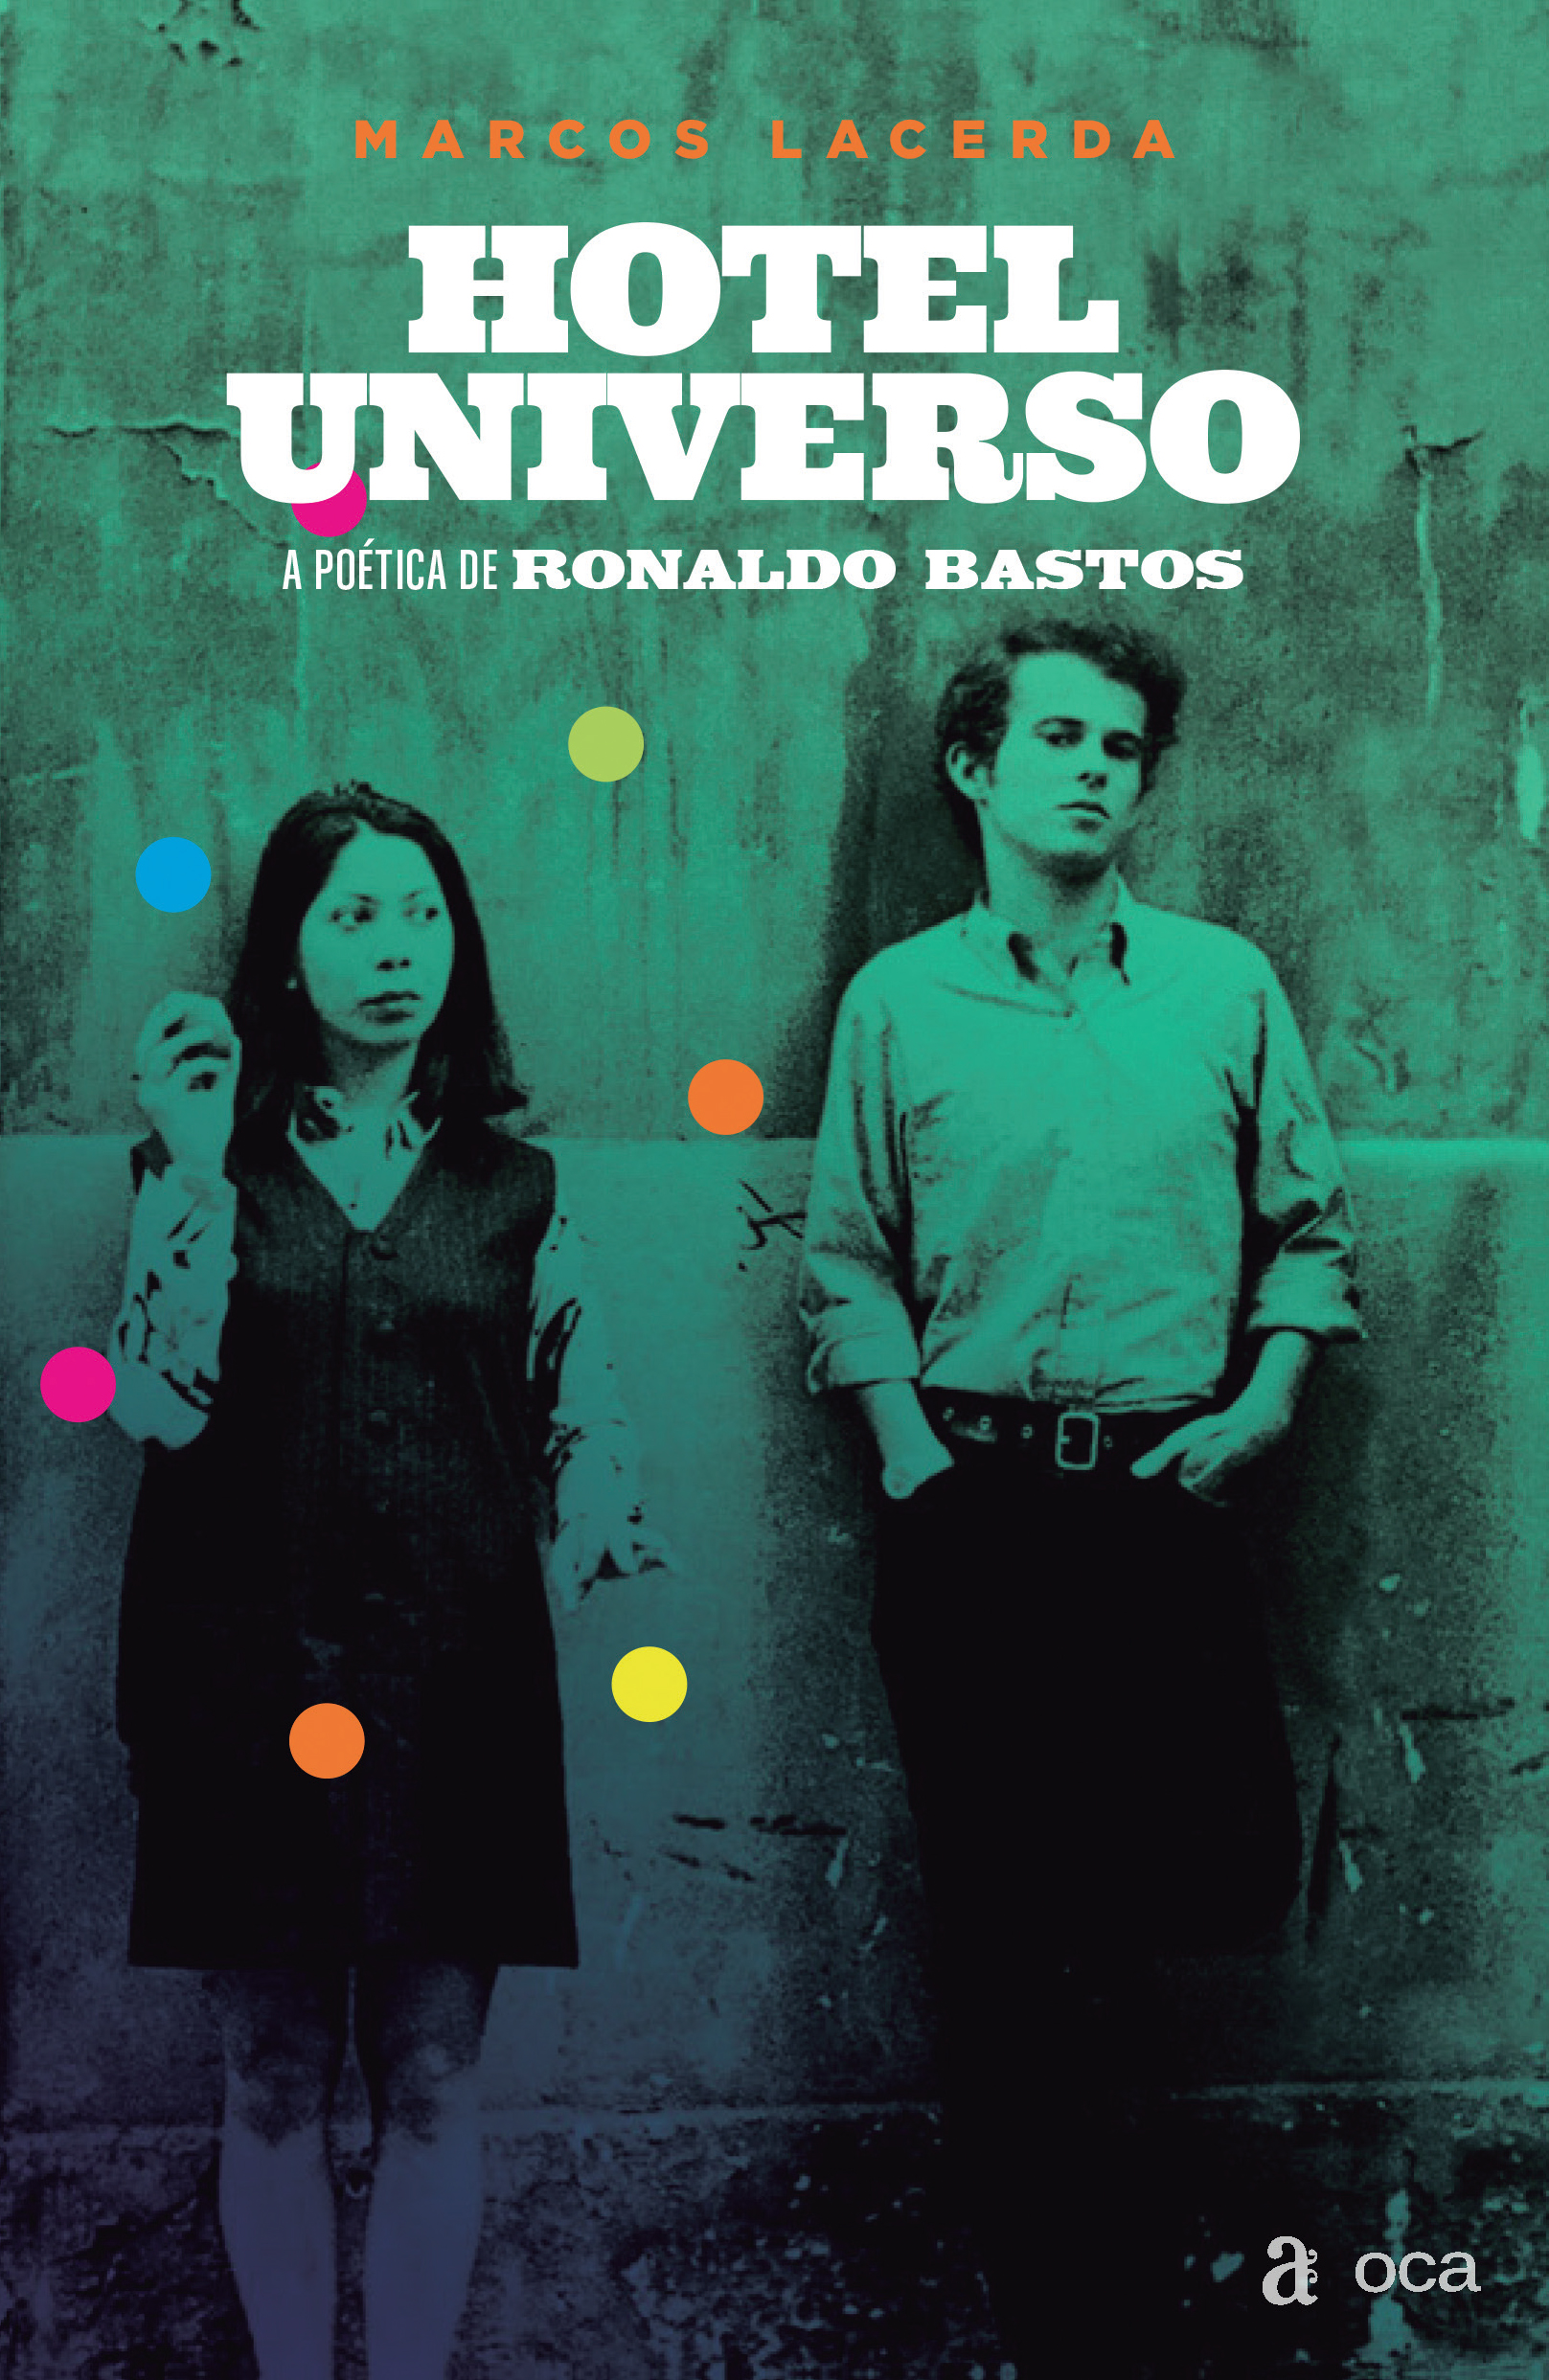
\includegraphics[width=45mm]{./imgs/universo.jpg}
\end{center}

\hspace*{-2cm}\_\_\_\_\_\_\_\_\_\_\_\_\_\_\_\_\_\_\_\_\_\_\_\_\_\_\_\_\_\_\_\_\_\_\_\_\_\_\_\_\_\_\_\_\_\_\_\_\_\_\_\_\_\_\_\_\_\_\_\_\_\_\_\_\_\_\_\_\_\_\_\_\_\_

\medskip

\noindent{}{\slsc{Hotel Universo}} traz uma antologia e uma análise do cancioneiro e da lírica de Ronaldo Bastos, realizada por Marcos Lacerda, importante crítico musical da nova geração. Um dos principais compositores da canção brasileira, Ronaldo Bastos foi um dos criadores do Clube da Esquina, que teve como expoentes artistas do porte de Milton Nascimento e Lô Borges, e suas canções foram gravadas por nomes como Caetano Veloso, Elis Regina e Tom Jobim.

%\hspace{.5cm}
\vfill

\hspace*{-.4cm}\begin{minipage}[c]{0.90\linewidth}
\small{
{\Formular{\textbf{
\hspace*{-.1cm}Título: Hotel Universo – a poética de Ronaldo Bastos\\
Autor: Marcos Lacerda\\ 
Editora: Azougue\\
Páginas: 174\\
Formato: 14x21cm\\
Preço: R\$ 39,00\\
ISBN: 978-85-7920-227-8
}}}}
\end{minipage}

\pagebreak

\hspace{.5cm}

\begin{center}
\hspace*{-2.5cm}\raisebox{5.5cm}{\rotatebox[origin=t]{90}{\Formular{\textbf{Lançamento}}}}
\hspace*{2cm}
\includegraphics[width=45mm]{./imgs/tembeta.jpg}
\end{center}

\hspace*{-2cm}\_\_\_\_\_\_\_\_\_\_\_\_\_\_\_\_\_\_\_\_\_\_\_\_\_\_\_\_\_\_\_\_\_\_\_\_\_\_\_\_\_\_\_\_\_\_\_\_\_\_\_\_\_\_\_\_\_\_\_\_\_\_\_\_\_\_\_\_\_\_\_\_\_\_

\medskip

\noindent{}Grandes lideranças e pensadores indígenas estão reunidos em {\slsc{Tembetá}}. São seis entrevistas, feitas com Ailton Krenak, Álvaro Tukano, Biraci Yawanawá, Eliane Potiguara, Jaider Esbell e Sônia Guajajara. É o primeiro volume de uma série que busca traçar um panorama plural do pensamento indígena contemporâneo, potencializando a voz dos povos originários em detrimento de uma fictícia e embolorada história dos “conquistadores”.

%\hspace{.5cm}
\vfill

\hspace*{-.4cm}\begin{minipage}[c]{0.90\linewidth}
\small{
{\Formular{\textbf{
\hspace*{-.1cm}Título: Tembetá\\
Autor: Sergio Cohn e Idjahure Kadiwéu (org.)\\ 
Editora: Azougue\\
Páginas: 206\\
Formato: 14x21cm\\
Preço: R\$ 45,90\\
ISBN: 978-85-7920-228-5
}}}}
\end{minipage}


\pagebreak

\hspace{.5cm}

\begin{center}
\hspace*{-.5cm}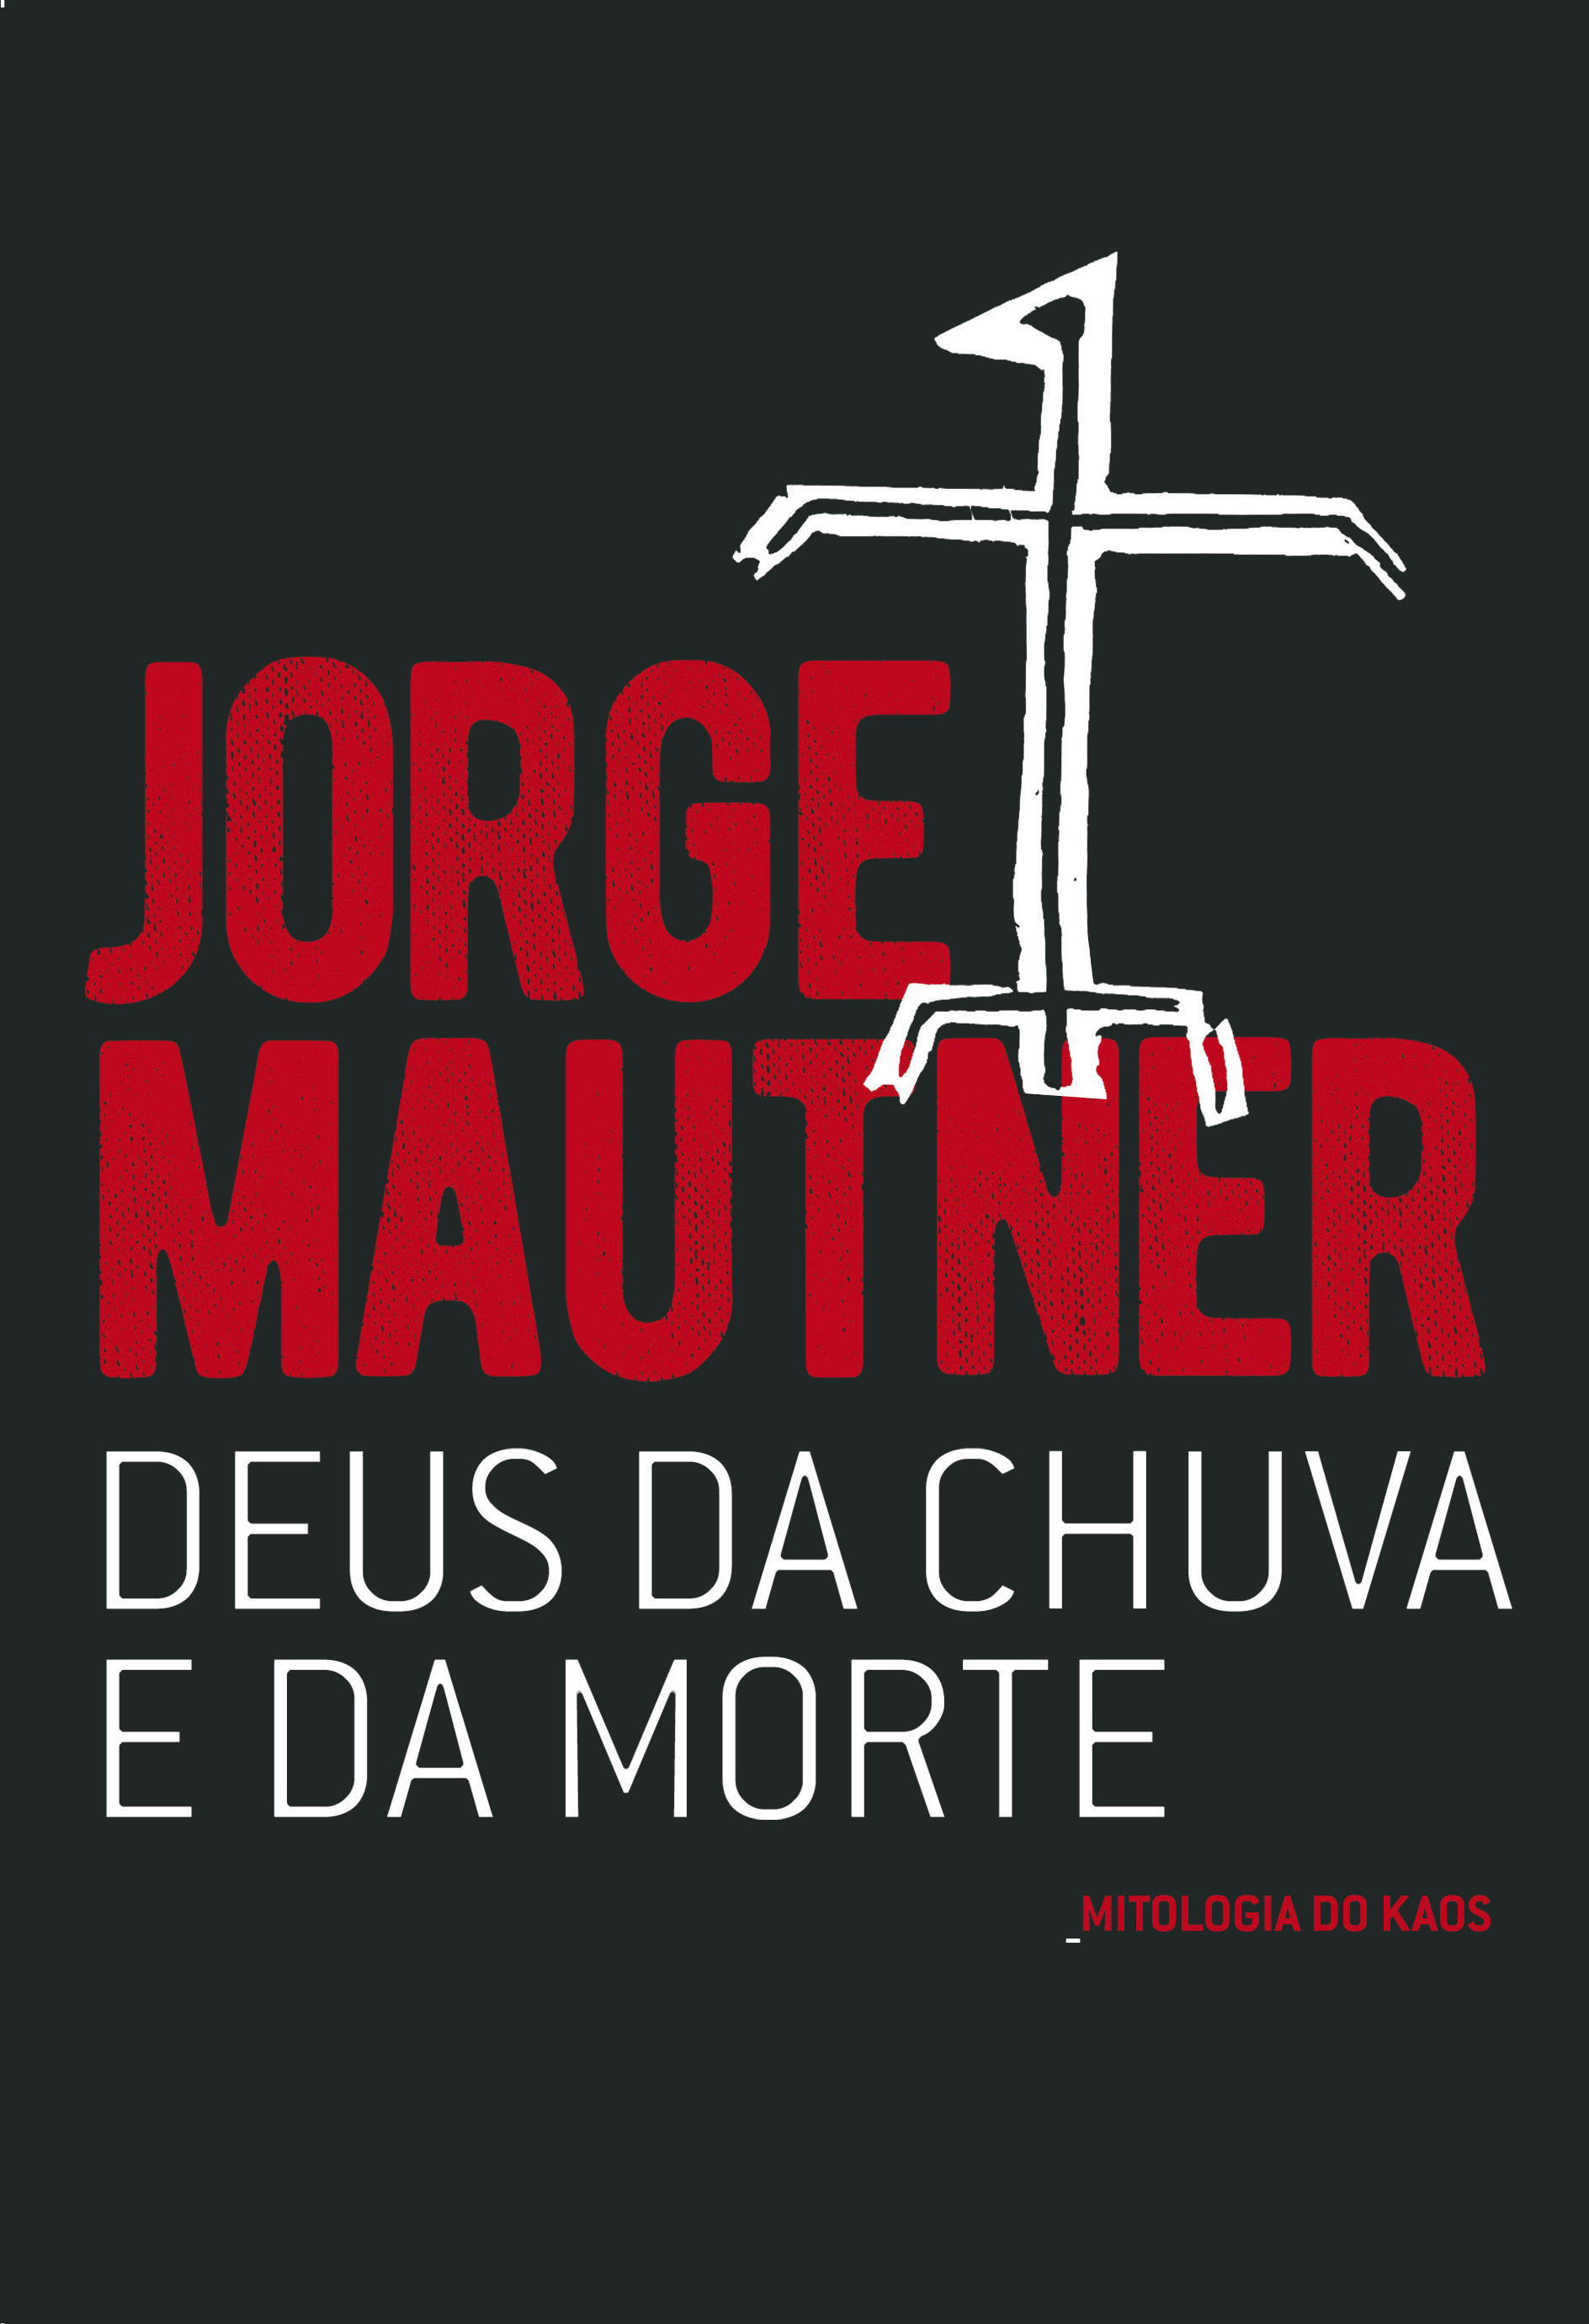
\includegraphics[width=47mm]{./imgs/mautner.jpg}
\end{center}

\hspace*{-2cm}\_\_\_\_\_\_\_\_\_\_\_\_\_\_\_\_\_\_\_\_\_\_\_\_\_\_\_\_\_\_\_\_\_\_\_\_\_\_\_\_\_\_\_\_\_\_\_\_\_\_\_\_\_\_\_\_\_\_\_\_\_\_\_\_\_\_\_\_\_\_\_\_\_\_

\medskip

\noindent{}Publicado originalmente em 1962, {\slsc{Deus da Chuva e da Morte}}, livro de estreia de Jorge Mautner, alcançou grande repercussão tanto de crítica como de público, conquistando o Prêmio Jabuti daquele ano e o consagrando como um dos autores mais singulares da literatura brasileira da época.

%\hspace{.5cm}
\vfill

\hspace*{-.4cm}\begin{minipage}[c]{0.90\linewidth}
\small{
{\Formular{\textbf{
\hspace*{-.1cm}Título: Mitologia do Kaos (Volume 1)\\
Autor: Jorge Mautner\\ 
Editora: Azougue\\
Páginas: 488\\
Formato: 16x23cm\\
Preço: R\$ 59,90\\
ISBN: 978-85-7920-234-6
}}}}
\end{minipage}

\pagebreak

\hspace{.5cm}

\begin{center}
\hspace*{-2.5cm}\raisebox{5.5cm}{\rotatebox[origin=t]{90}{\Formular{\textbf{Lançamento}}}}
\hspace*{2cm}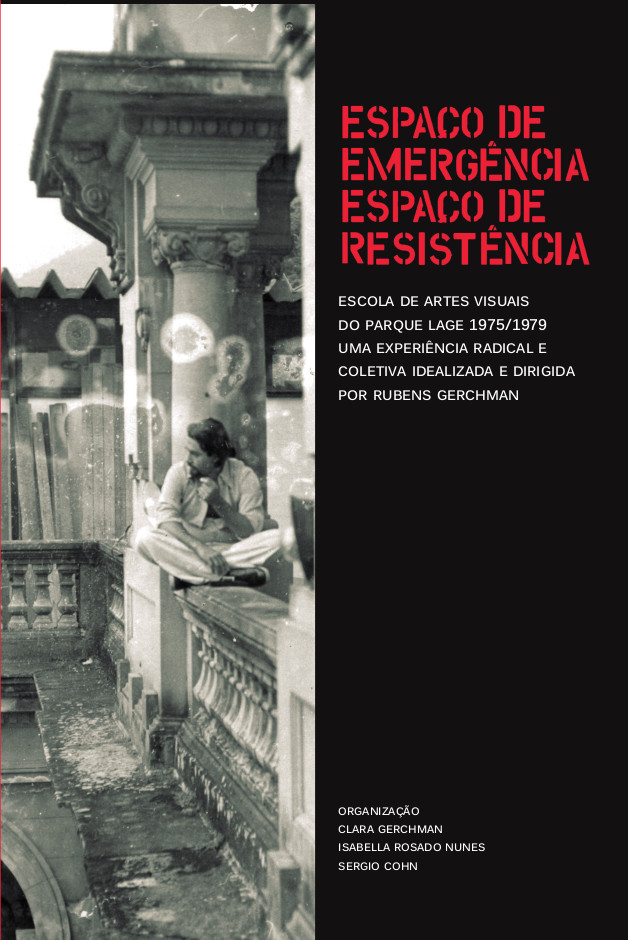
\includegraphics[width=45mm]{./imgs/lage.jpeg}
\end{center}

\hspace*{-2cm}\_\_\_\_\_\_\_\_\_\_\_\_\_\_\_\_\_\_\_\_\_\_\_\_\_\_\_\_\_\_\_\_\_\_\_\_\_\_\_\_\_\_\_\_\_\_\_\_\_\_\_\_\_\_\_\_\_\_\_\_\_\_\_\_\_\_\_\_\_\_\_\_\_\_

\medskip

\noindent{}Este livro reúne as falas de Gerchman, documentos, cartas,
recortes de jornal, material gráfico e uma série de 25 depoimentos com
protagonistas da época que permitem
um mergulho profundo na \scalebox{.8}{EAV} da segunda metade da década de 70. Acrescido de 3 ensaios, {\slsc{Espaço de emergência}} penetra no que foi o maior exercício experimental de liberdade no ensino e na vivência de arte no Brasil.

\hspace{.5cm}
\vfill

\hspace*{-.4cm}\begin{minipage}[c]{1\linewidth}
\small{
{\Formular{\textbf{
\hspace*{-.1cm}Título: Espaço de emergência, espaço de resistência: Escola de Artes Visuais do Parque Lage 1975-1979\\ %, uma experiência radical e coletiva idealizada e dirigida por Rubens Gerchman\\
Autor: Clara Gerchman, Isabella Rosado Nunes e Sergio Cohn (org.)\\ 
Editora: Azougue\\
Páginas: 154\\
Formato: 14x21cm\\
Preço: R\$ 39,90\\
ISBN: 978-85-7920-226-1
}}}}
\end{minipage}


\pagebreak
